% A Tour of Pollis — draft 1 (3 October 2026; called the brochure until 10 October 2026)
% Compile with: latexmk -pdf pollis_tour.tex
\documentclass[10pt,a4paper]{article}

\usepackage[a4paper,left=17mm,right=17mm,top=15mm,bottom=17mm,footskip=8mm]{geometry}
\usepackage[T1]{fontenc}
\usepackage[default,semibold]{sourcesanspro}
\usepackage{microtype}
\usepackage{graphicx}
\usepackage[table]{xcolor}
\usepackage{tikz}
\usetikzlibrary{positioning,calc,arrows.meta}
\usepackage[most]{tcolorbox}
\usepackage{fontawesome5}
\usepackage{tabularx}
\usepackage{enumitem}
\usepackage{fancyhdr}
\usepackage{qrcode}
\usepackage[hidelinks]{hyperref}

\graphicspath{{images/}}

% ---------------------------------------------------------------- placeholders
% Change these in one place. Placeholders print in orange so they are easy to spot.
\newcommand{\todo}[1]{\textcolor{orange}{\textbf{[#1]}}}
\newcommand{\downloadlink}{\href{https://github.com/saragga/pollis/releases/latest}{github.com/saragga/pollis/releases/latest}}
\newcommand{\contactemail}{\href{mailto:contact@pollis.org}{contact@pollis.org}}
\newcommand{\tourdate}{15 October 2026}
\newcommand{\sourcelink}{github.com/saragga/pollis}

% ---------------------------------------------------------------- colours
\definecolor{navy}{HTML}{1C3A5E}
\definecolor{pblue}{HTML}{3B78B5}
\definecolor{amber}{HTML}{F2B33D}
\definecolor{deepamber}{HTML}{D9902A}
% A Julia package name, in the Pollis yellow
\newcommand{\pkg}[1]{\textbf{\textcolor{deepamber}{#1}}}
\definecolor{cream}{HTML}{FFF3D6}
\definecolor{pale}{HTML}{EEF3F9}
\definecolor{ink}{HTML}{2A2F36}
\definecolor{logonavy}{HTML}{173D63}
\definecolor{logodark}{HTML}{C98A1E}
\definecolor{logoamber}{HTML}{F2B446}
\definecolor{logocream}{HTML}{FEEFD2}
\definecolor{soft}{HTML}{5E6773}
\color{ink}

% ---------------------------------------------------------------- layout helpers
\setlength{\parindent}{0pt}
\setlength{\parskip}{4pt}
\setlist{nosep,leftmargin=*,itemsep=2pt}

\pagestyle{fancy}
\fancyhf{}
\renewcommand{\headrulewidth}{0pt}
\fancyfoot[L]{\footnotesize\color{soft}\textbf{Pollis}\enspace Bright Insights through Statistical Learning, Simulation and Optimisation}
\fancyfoot[R]{\footnotesize\color{soft}\thepage}

% The Pollis logo, redrawn so it prints sharply at any size
\newcommand{\pollislogo}[1]{%
  % geometry traced from the 512 x 512 logo file
  \begin{tikzpicture}[x=#1/512,y=-#1/512,baseline=(current bounding box.center)]
    \fill[logonavy] (0,0) rectangle (512,512);
    \fill[logodark] (36,422) -- (104,256) -- (172,422) -- cycle;
    \fill[logoamber] (104,422) -- (203,180) -- (302,422) -- cycle;
    \fill[logocream] (203,422) -- (339,89) -- (476,422) -- cycle;
  \end{tikzpicture}}

% Page heading: kicker, title, one-line promise
\newcommand{\pageheading}[3]{%
  {\color{deepamber}\small\bfseries\MakeUppercase{#1}}\par\vspace{1pt}
  {\color{navy}\fontsize{22}{26}\selectfont\bfseries #2}\par\vspace{3pt}
  {\color{soft}\large #3}\par\vspace{6pt}}

\newcommand{\subhead}[1]{{\color{navy}\large\bfseries #1}\par\vspace{2pt}}

% Text boxes
\newtcolorbox{pbox}[2][]{enhanced, colback=pale, colframe=amber, boxrule=0pt,
  leftrule=3pt, sharp corners, left=7pt, right=7pt, top=6pt, bottom=6pt,
  fontupper=\small\raggedright, before upper={{\color{navy}\normalsize\bfseries #2}\par\smallskip}, #1}
\newtcolorbox{nbox}[2][]{enhanced, colback=navy, colframe=navy, boxrule=0pt,
  sharp corners, left=8pt, right=8pt, top=7pt, bottom=7pt, coltext=white,
  fontupper=\small, before upper={{\color{amber}\normalsize\bfseries #2}\par\smallskip}, #1}

% Screenshot frame
\newcommand{\shot}[2][\linewidth]{%
  \tcbox[enhanced, colback=black, colframe=black!70, boxrule=0.4pt, arc=2pt,
    left=0pt,right=0pt,top=0pt,bottom=0pt, boxsep=0pt]{\includegraphics[width=\dimexpr#1-1pt\relax]{#2}}}
\newcommand{\shotcap}[1]{{\footnotesize\color{soft}#1\par}}
% A list icon, centred in a fixed width so icons of different widths line up
\newcommand{\listicon}[1]{\makebox[1.25em][c]{\color{deepamber}#1}}
% A card with a title, a tag, a subtitle and a body (Reports, Practice, Collaboration)
\newcommand{\collabmode}[4]{%
  \begin{tcolorbox}[enhanced, colback=white, colframe=navy, boxrule=0.6pt, arc=3pt,
     left=7pt,right=7pt,top=7pt,bottom=7pt, fontupper=\small\raggedright]
   {\color{navy}\large\bfseries #1}\hfill{\footnotesize\color{soft}#2}\par\vspace{2pt}
   {\color{deepamber}\bfseries #3}\par\vspace{4pt}
   #4
  \end{tcolorbox}}

% Numbered markers for the annotated panel
\newcommand{\mk}[1]{\tikz[baseline=(c.base)]\node[circle, fill=amber, text=navy,
  font=\footnotesize\bfseries, inner sep=1.2pt, minimum size=4.2mm](c){#1};}

\begin{document}

% =====================================================================
% PAGE 1 — COVER
% =====================================================================
\thispagestyle{empty}
\begin{minipage}[c]{24mm}\pollislogo{22mm}\end{minipage}%
\begin{minipage}[c]{0.84\linewidth}
  {\color{navy}\fontsize{40}{42}\selectfont\bfseries Pollis}\par\vspace{2pt}
  {\color{navy}\Large Bright Insights through Statistical Learning, Simulation and Optimisation}
\end{minipage}

\vspace{7mm}
\noindent\begin{minipage}[t]{0.62\linewidth}\vspace{0pt}
{\color{navy}\fontsize{30}{34}\selectfont\bfseries From eureka\\ to evidence.}\par\vspace{3mm}
{\color{deepamber}\Large Had an idea? Pollis helps you test it, in code you own,\\ and then improve and expand it.}
\end{minipage}\hfill
\begin{minipage}[t]{0.27\linewidth}\vspace{0pt}
\begin{tcolorbox}[enhanced, colback=white, colframe=amber, boxrule=0pt, leftrule=2pt, sharp corners,
  left=7pt, right=0pt, top=1pt, bottom=1pt, fontupper=\footnotesize]
{\color{navy}\bfseries Contents}\par\smallskip
\renewcommand{\arraystretch}{1.0}
\begin{tabular}{@{}r@{\enspace}l@{}}
{\color{deepamber}\bfseries 1} & From eureka to evidence\\
{\color{deepamber}\bfseries 2} & What Pollis is\\
{\color{deepamber}\bfseries 3} & Inside a panel\\
{\color{deepamber}\bfseries 4} & Teaching built in\\
{\color{deepamber}\bfseries 5} & Coverage\\
{\color{deepamber}\bfseries 6} & Customisation\\
{\color{deepamber}\bfseries 7} & Extensions\\
{\color{deepamber}\bfseries 8} & Replication and Workflows\\
{\color{deepamber}\bfseries 9} & Reports\\
{\color{deepamber}\bfseries 10} & Monitor\\
{\color{deepamber}\bfseries 11} & Collaboration\\
{\color{deepamber}\bfseries 12} & Free and open\\
{\color{deepamber}\bfseries 13} & Everything in Pollis
\end{tabular}
\end{tcolorbox}
\end{minipage}

\vspace{6mm}
\begin{minipage}{0.86\linewidth}\large
A free, open-source desktop environment to explore data, build models, run
simulations and solve optimisation problems: from your first click to your own code.
\end{minipage}

\vspace{8mm}
\shot{welcome_cover.jpg}

\vspace{8mm}
\begin{tcbraster}[raster columns=4, raster equal height, raster column skip=3mm,
  enhanced, colback=pale, colframe=pale, boxrule=0pt, sharp corners,
  left=5pt,right=5pt,top=6pt,bottom=6pt, fontupper=\small\raggedright]
\begin{tcolorbox}{\color{deepamber}\Large\faMousePointer}\par\smallskip
  {\color{navy}\bfseries Start by clicking}\par Choose a method, fill in a few boxes, run the example.\end{tcolorbox}
\begin{tcolorbox}{\color{deepamber}\Large\faCode}\par\smallskip
  {\color{navy}\bfseries Keep the code}\par Every panel writes readable Julia code that is yours.\end{tcolorbox}
\begin{tcolorbox}{\color{deepamber}\Large\faGraduationCap}\par\smallskip
  {\color{navy}\bfseries Learn good practice}\par Which method, how to check it, where to read more.\end{tcolorbox}
\begin{tcolorbox}{\color{deepamber}\Large\faLayerGroup}\par\smallskip
  {\color{navy}\bfseries All in one place}\par 656 procedures in 203 panels, from statistics to optimal control.\end{tcolorbox}
\end{tcbraster}

\vfill
\begin{minipage}[b]{0.8\linewidth}
{\color{soft}\small
\textbf{Free}\enspace·\enspace\textbf{Open source} (AGPL 3.0)\enspace·\enspace\textbf{Windows, macOS, Linux}\par\vspace{2pt}
\textcopyright\ 2026 Antonio Saragga Seabra\enspace·\enspace Licensed under \href{https://creativecommons.org/licenses/by-sa/4.0/}{CC BY-SA 4.0}\enspace·\enspace\tourdate}
\end{minipage}

\newpage
% =====================================================================
% PAGE 2 — WHAT POLLIS IS
% =====================================================================
\pageheading{What Pollis is}{Data and a question? Start here.}
  {One desktop application for the whole job, organised by what you want to do.}

\begin{minipage}{\linewidth}\large
Pollis is for anyone who has data and a question. You pick a method from a menu,
fill in a few boxes, and Pollis gives you working code that produces the result,
together with advice on what a careful analyst does next.
You do not need to program to start.
\end{minipage}

\vspace{2mm}
Behind the menus are the Julia language and 289 open-source Julia packages.
Pollis looks and works like a familiar code editor, with five extra, curated menus:
\textbf{Explore}, \textbf{Model}, \textbf{Simulate}, \textbf{Optimise} and \textbf{Compose}.

\vspace{2mm}
\newcommand{\stepbox}[4]{%
  \begin{tcolorbox}[enhanced, colback=white, colframe=navy, boxrule=0.6pt, arc=3pt,
     left=4pt,right=4pt,top=4pt,bottom=4pt, fontupper=\footnotesize\raggedright,
     title={\faIcon{#1}\enspace #2}, fonttitle=\bfseries\normalsize, colbacktitle=navy, coltitle=white,
     toptitle=2pt, bottomtitle=2pt]
   {\color{deepamber}\bfseries #3}\par\smallskip #4
  \end{tcolorbox}}
\begin{tcbraster}[raster columns=5, raster equal height, raster column skip=2.5mm]
\stepbox{search}{Explore}{What do my data look like?}{%
  Bring in data from finance, economics and AI libraries, Excel, CSV or SQL.
  Thirty-five plot types, from scatter plots to Sankey diagrams and maps.
  Descriptive statistics, outliers, missing data.}
\stepbox{chart-line}{Model}{What explains it?}{%
  Regression with robust inference, generalised linear models, time series,
  survival analysis, Bayesian inference, machine learning, neural networks and text analysis.}
\stepbox{dice}{Simulate}{What could happen?}{%
  Monte Carlo and Markov chain Monte Carlo, bootstrap, stochastic differential
  equations, agent-based models and network models.}
\stepbox{bullseye}{Optimise}{What is the best decision?}{%
  Linear, convex and nonlinear programming, global and Bayesian optimisation,
  optimal control, Markov decision processes and reinforcement learning.}
\stepbox{layer-group}{Compose}{How do I put it all together?}{%
  Replications of classic papers, new methods as packages, workflows, reports,
  collaboration, coding agents with their skills, and local reasoning models.}
\end{tcbraster}


\vspace{0mm}
% Numbers strip
\newcommand{\bignum}[2]{\begin{minipage}[t]{0.24\linewidth}\centering
  {\color{navy}\fontsize{22}{24}\selectfont\bfseries #1}\par\vspace{1pt}{\footnotesize\color{soft}#2}\end{minipage}}
\noindent\bignum{5}{curated menus}\hfill\bignum{203}{method panels}%
\hfill\bignum{656}{procedures}\hfill\bignum{289}{open-source Julia packages}

\vspace{2mm}
\begin{minipage}[t]{0.56\linewidth}\vspace{0pt}
\begin{pbox}{Ideas you could test this afternoon}
\begin{itemize}
  \item[\color{deepamber}\faCity] \textbf{Can mild preferences split a whole city?} Neighbours who only want a few people like them nearby.
    \emph{Agent-based Schelling model.}
  \item[\color{deepamber}\faProjectDiagram] \textbf{Does a rumour spread like a virus?} Run an epidemic model on a social network.
    \emph{Network SIR simulation.}
  \item[\color{deepamber}\faHeartbeat] \textbf{How fast is an outbreak growing right now?} Estimate the reproduction number from daily case counts.
    \emph{Bayesian renewal model.}
  \item[\color{deepamber}\faUniversity] \textbf{Did the interest-rate rise work?} Trace a policy shock through inflation and output.
    \emph{VAR impulse responses.}
  \item[\color{deepamber}\faRobot] \textbf{Can a computer teach itself to balance a pole?} Watch it learn by trial and error.
    \emph{Reinforcement learning.}
\end{itemize}
\end{pbox}
\end{minipage}\hfill
\begin{minipage}[t]{0.41\linewidth}\vspace{0pt}
\begin{pbox}{Who is it for?}
\textbf{Students} encountering a method for the first time, who want to see it in action and explore what happens when assumptions change.\par\smallskip
\textbf{Lecturers} who want to teach with real, runnable code and the literature behind it.\par\smallskip
\textbf{Researchers} who want classical statistics, machine learning, simulation and optimisation without switching tools.\par\smallskip
\textbf{Authors} of books and reports who want to illustrate and enhance their work with Pollis, using customised Views and panels: for example, a View that follows the text, chapter by chapter.
\end{pbox}
\end{minipage}

\vspace{3mm}
\begin{tcolorbox}[enhanced, colback=pale, colframe=pale, sharp corners, boxrule=0pt,
  left=6pt,right=6pt,top=4pt,bottom=4pt, fontupper=\small]
\begin{minipage}[c]{0.62\linewidth}
\faToolbox\enspace\textbf{Toolboxes} add whole fields to the menus, one click to install.
\par\vspace{3pt}\textbf{Julia packages} do the computing. They are the open-source libraries such as \pkg{GLM.jl} or \pkg{Turing.jl}. Every panel's code calls them, and Pollis installs them into Julia when a panel needs them.\par\vspace{3pt}
\textbf{Toolbox extensions} are Pollis add-ons. Each one adds a menu of ready-made panels for a field, installed with one click from the Extensions pane. Those panels in turn run on Julia packages. You choose which panels to add, and where.\par\vspace{3pt}
Three are ready from the start:\par\vspace{3pt}
\textbf{Financial Econometrics}, including ARIMAX, VAR/VECM, GARCH, regime switching and advanced time-series forecasting.\par\vspace{2pt}
\textbf{Economics}, including DSGE, heterogeneous-agent models, continuous-time macro-finance and game theory.\par\vspace{2pt}
\textbf{Mathematical Core}, including symbolic maths, linear algebra, differential equations and solvers.\par\vspace{3pt}
Many more are on the way. Creating a new toolbox is quick and easy: just package existing procedure panels into a ready-to-use collection. Toolboxes make it simple to share your work, extend Pollis, and make your methods available to the wider community.
\end{minipage}\hfill
\begin{minipage}[c]{0.33\linewidth}
\shot{toolboxes_pane}
\end{minipage}
\end{tcolorbox}

\newpage
% =====================================================================
% PAGE 3 — ANATOMY OF A PANEL  (message 1)
% =====================================================================
\pageheading{Inside a panel}{Start by clicking, end with code you own.}
  {Each of the 203 panels brings together one or more methods and their procedures, with everything you need around them.}

\begin{minipage}[t]{0.60\linewidth}\vspace{0pt}
\begin{tikzpicture}
  \node[inner sep=0, anchor=south west] (img) {\shot[\linewidth]{glm}};
  \begin{scope}[x={(img.south east)}, y={(img.north west)}]
    % positions are fractions of the screenshot (GLM panel, 1310 x 1208 px)
    \foreach \n/\yy in {1/91, 2/228, 3/345, 4/458, 6/830, 7/1056, 8/1116, 9/1178}
      \node[circle, fill=amber, text=navy, font=\footnotesize\bfseries, inner sep=1.2pt,
            minimum size=4.6mm, draw=navy, line width=0.4pt] at (0.045, {1-\yy/1208}) {\n};
    % 5 sits on the tab row, mirroring the left markers
    \node[circle, fill=amber, text=navy, font=\footnotesize\bfseries, inner sep=1.2pt,
          minimum size=4.6mm, draw=navy, line width=0.4pt] at (0.97, {1-458/1208}) {5};
  \end{scope}
\end{tikzpicture}
\shotcap{The Generalised Linear Models panel. Choosing a family, a link or a kind of inference (Standard, HC0--HC3, HAC or Clustered) rewrites the example code.}
\end{minipage}\hfill
\begin{minipage}[t]{0.37\linewidth}\vspace{0pt}\small
\setlength{\parskip}{3.2pt}
\mk1\enspace\textbf{Powered by.} The open-source Julia packages behind the method (here: \pkg{GLM.jl} and \pkg{\mbox{CovarianceMatrices.jl}}) working together, with links. A tick when they are installed, or a one-click \emph{Install}.

\mk2\enspace\textbf{Key Points.} The method in a few lines.

\mk3\enspace\textbf{Decision Table.} Which variant to use, and when.

\mk4\enspace\textbf{Your choices.} Family, link function and kind of inference: tabs and drop-down lists.

\mk5\enspace\textbf{Your own tab.} Click \textbf{+} to add a tab of your own, with your own code.

\mk6\enspace\textbf{Example code.} Real Julia code that follows your choices, with comments.

\mk7\enspace\textbf{Run it your way.} Edit or copy the code, or send it directly to the Julia REPL, the Editor, or a Jupyter or Pluto notebook.

\mk8\enspace\textbf{Next Steps.} Ready-made code to Visualise, Diagnose, Predict, Compare and Interpret the fitted model.

\mk9\enspace\textbf{Learn More.} Local wikis, notebook tutorials, video tutorials and references.
\end{minipage}

\vspace{4mm}
\begin{tikzpicture}
  \node[inner sep=0, anchor=south west] (img) {\shot[\linewidth]{glm_added_tab}};
  \begin{scope}[x={(img.south east)}, y={(img.north west)}]
    % position is a fraction of the screenshot (added tab, 1900 x 467 px), on the tab row
    \node[circle, fill=amber, text=navy, font=\footnotesize\bfseries, inner sep=1.2pt,
          minimum size=4.6mm, draw=navy, line width=0.4pt] at (0.024, {1-101/467}) {5};
  \end{scope}
\end{tikzpicture}\par\smallskip
\shotcap{A tab of your own. Click \textbf{+}, name the tab and write any Julia code in it; it is kept with the panel, ready for next time. Its $\times$ removes it.}

\vspace{6mm}
\begin{minipage}[t]{0.485\linewidth}\vspace{0pt}
\begin{pbox}{Do I need to know how to program?}
No, not to start. Fill in the boxes and run the example. Reading the code that Pollis
writes is the easiest way to learn; changing it is the next step.
Julia installs from the Welcome page. When a panel needs a package, Pollis installs it
for you, with your agreement, in one click.
\end{pbox}
\end{minipage}\hfill
\begin{minipage}[t]{0.485\linewidth}\vspace{0pt}
\begin{pbox}{Every example runs as shipped}
Each example comes with its own data: simulated, or a well-known real dataset from the
companion package \pkg{PollisDatasets.jl}. Press \emph{Julia REPL} and it runs.
Then replace the example data with yours.
\end{pbox}
\end{minipage}

\vspace{3mm}
\begin{nbox}{Not a black box}
Pollis is not a point-and-click statistics package that hides what it does. Every result
comes with the code that produced it. You can read it, change it, rerun it and share it,
so a colleague, a referee or a student can check exactly what was done.
The path from menus to programming is a short one.
\end{nbox}

\newpage
% =====================================================================
% PAGE 4 — GOOD PRACTICE BUILT IN  (message 2)
% =====================================================================
\pageheading{Teaching built in}{More than tools: it teaches good practice.}
  {Pollis helps you choose a method, check it and understand it.}

\subhead{\color{deepamber}1\enspace\color{navy}Choose: which method, and when?}
\shot{ts_decision}\par\vspace{2pt}
\shotcap{The Decision Table of the Time-Series Forecasting panel: what kind of data each model suits, and when to use it, in plain words.}

\vspace{4mm}
\subhead{\color{deepamber}2\enspace\color{navy}Check: what does a careful analyst do next?}
\begin{minipage}[t]{0.54\linewidth}\vspace{0pt}
\shot{diagnose}\par\vspace{2pt}
\shotcap{Next Steps \textrightarrow{} Diagnose, after a linear regression: residuals against fitted values, a residual Q--Q plot, leverage and Cook's distance.}
\vspace{3mm}
\small After fitting a model, \textbf{Next Steps} offers ready-made code for five things
a careful analyst does: \textbf{Visualise} the fit, \textbf{Diagnose} its assumptions,
\textbf{Predict} new values, \textbf{Compare} it with other models and \textbf{Interpret}
the results. One click sends the code to the Julia REPL, and the plot appears.
\end{minipage}\hfill
\begin{minipage}[t]{0.42\linewidth}\vspace{0pt}
\shot{plot_kde}\par\vspace{2pt}
\shotcap{Next Steps \textrightarrow{} Visualise \textrightarrow{} Density Overlay: a smooth KDE curve on top of a histogram.}
\end{minipage}

\vspace{5mm}
\subhead{\color{deepamber}3\enspace\color{navy}Learn: where can I discover more?}
\begin{minipage}[t]{0.485\linewidth}\vspace{0pt}\small\raggedright
\textbf{Learn More} is not merely documentation, but a place for discovery and intellectual
inspiration. Go beyond the standard information and discover new knowledge, ideas and
perspectives. Explore inspiring cases and practical examples, and let them inspire your own
analyses. Learn More brings together:
\begin{itemize}
  \item[\listicon{\faBook}] \textbf{Local wikis} that go beyond the method, to the ideas, fields and questions around it;
  \item[\listicon{\faClipboardList}] \textbf{Notebook tutorials} that tell a story, with comments, images and code you can run and change at your leisure: a rich teaching tool;
  \item[\listicon{\faPlayCircle}] \textbf{Video tutorials}, from high-performance computing in Julia to MIT's \emph{Introduction to Computational Thinking}: many topics, for many audiences;
  \item[\listicon{\faLink}] \textbf{References}: the papers and books behind the method and its packages.
\end{itemize}
\end{minipage}\hfill
\begin{minipage}[t]{0.485\linewidth}\vspace{0pt}
\begin{pbox}{Method, code, interpretation, literature}
Most software runs the method you ask for. Pollis also connects it to the choice
that came before (the Decision Table), the checks that come after (Next Steps) and
the knowledge, ideas and literature around it (Learn More). That is the teaching a good supervisor does,
built into every panel.
\end{pbox}
\end{minipage}

\newpage
% =====================================================================
% PAGE 5 — ONE PLACE, THE SIZE YOU NEED  (message 3)
% =====================================================================
\pageheading{Coverage}{The whole job in one place, at the size you need.}
  {From classical statistics to machine learning, simulation and operations research.}

{\small
\renewcommand{\arraystretch}{1.25}
\rowcolors{2}{white}{white}
\begin{tabularx}{\linewidth}{@{}>{\raggedright\arraybackslash}X@{\hspace{3mm}}>{\raggedright\arraybackslash}X@{\hspace{3mm}}>{\raggedright\arraybackslash}X@{\hspace{3mm}}>{\raggedright\arraybackslash}X@{}}
\cellcolor{navy}\color{white}\bfseries Explore\hfill\color{amber}49 &
\cellcolor{navy}\color{white}\bfseries Model\hfill\color{amber}69 &
\cellcolor{navy}\color{white}\bfseries Simulate\hfill\color{amber}26 &
\cellcolor{navy}\color{white}\bfseries Optimise\hfill\color{amber}52 \\[1pt]
\footnotesize
Data libraries\newline
Excel, CSV and SQL\newline
35 plot types, from box plots to Sankey diagrams, choropleth maps and voxel plots\newline
Descriptive statistics\newline
Anomaly and novelty detection\newline
Missing data, interpolation
&
\footnotesize
Linear models with robust inference, 2SLS, GMM\newline
Generalised and mixed models\newline
Time-series forecasting, state space\newline
Survival analysis\newline
Bayesian analysis\newline
Trees, ensembles, clustering\newline
Neural networks, transformers\newline
Text: topic models, BERT, LLMs
&
\footnotesize
Random and quasi-random numbers\newline
Markov chain, sequential and multilevel Monte Carlo\newline
Bootstrap\newline
Probabilistic programming\newline
Stochastic differential equations\newline
Agent-based models\newline
Network models
&
\footnotesize
Linear, quadratic, conic and nonlinear programming\newline
Global, Bayesian and evolutionary optimisation\newline
Multi-objective, robust and stochastic optimisation\newline
Optimal control\newline
Reinforcement learning, including AlphaZero
\end{tabularx}}

\vspace{4mm}
\begin{tcolorbox}[enhanced, colback=pale, colframe=pale, sharp corners, boxrule=0pt,
  left=7pt,right=7pt,top=6pt,bottom=6pt]
{\color{navy}\bfseries\faDatabase\enspace Data at hand.}\enspace\small
Panels read data from
\textbf{Yahoo Finance}, \textbf{Alpha Vantage}, \textbf{US SEC EDGAR}, \textbf{FRED}, the \textbf{ECB},
the \textbf{IMF}, the \textbf{World Bank}, the \textbf{Kenneth French Data Library},
\textbf{Hugging Face} and \textbf{Kaggle}, as well as \textbf{Excel}, \textbf{CSV} and \textbf{SQL}.
A built-in database and a Databases pane cover DuckDB, PostgreSQL and SQLite.
\end{tcolorbox}

\vspace{3mm}
\begin{minipage}[t]{0.55\linewidth}\vspace{0pt}
\shot{hf_browser}\par\vspace{2pt}
\shotcap{Browse Hugging Face models by task, framework and author, sorted by trend, likes, downloads or date, without leaving Pollis.}
\end{minipage}\hfill
\begin{minipage}[t]{0.41\linewidth}\vspace{0pt}
\begin{pbox}{Models, not just data}
\textbf{Compose \textrightarrow{} Local Models} gets models from Hugging Face and Kaggle, and lists the models on this computer, which Pollis runs with the llama.cpp that comes with it.
Example code covers multimodal, language, vision, audio, tabular, reinforcement-learning,
graph and embedding models.
\end{pbox}
\vspace{2mm}
\shot{databases}\par\vspace{2pt}
\shotcap{The built-in database: 54 real data sets, ready to query and to browse as a table.}
\end{minipage}

\vspace{6mm}
\begin{pbox}{Private by design \hspace{1.5mm}{\color{deepamber}\faLock}}
\textbf{No telemetry, no cloud:} Pollis collects no usage data and runs no cloud service of its
own, so your data and models stay on your computer.
\textbf{Your keys stay safe:} keys for Hugging Face, Kaggle, FRED and Alpha Vantage, and the
contact e-mail EDGAR asks for, are kept in your system's secure store (Keychain on macOS,
Credential Manager on Windows). They are passed only to the running Julia session and never
written into your code, notebooks or files, so a script you share never leaks a key.
\end{pbox}

\newpage
% =====================================================================
% PAGE 6 — MAKE IT YOURS (customisation)
% =====================================================================
\pageheading{Customisation}{Make it yours.}
  {Shape Pollis around a course, a book, a research group or an institution.}

\begin{minipage}{\linewidth}\large
Most analysis software gives everyone the same menus. Pollis lets the people who teach,
write and research decide what their students and readers see, and still hands them
real code.
\end{minipage}

\vspace{5mm}
\newcommand{\level}[5]{%
  \begin{tcolorbox}[enhanced, colback=white, colframe=navy, boxrule=0.6pt, arc=3pt,
     left=7pt,right=7pt,top=7pt,bottom=7pt, fontupper=\small\raggedright]
   \begin{tikzpicture}[baseline=(n.base)]\node[circle, fill=amber, text=navy, font=\large\bfseries,
     minimum size=8mm, inner sep=0](n){#1};\end{tikzpicture}\enspace
   {\color{navy}\large\bfseries #2}\par\vspace{5pt}
   {\color{deepamber}\bfseries #3}\par\vspace{4pt}
   #4\par\vspace{6pt}
   {\footnotesize\color{soft}\faUser\enspace #5}
  \end{tcolorbox}}
\begin{tcbraster}[raster columns=3, raster equal height, raster column skip=3mm]
\level{1}{Views}{Choose what to show.}{%
  Select the panels you need and reshape the menu structure around them. Save the result as
  a named View: a course, a talk, a book.}{No programming needed}
\level{2}{Your panels}{Change the examples.}{%
  Edit a panel's example code to use your data, your variable names and your notation,
  and keep it, or add tabs of your own. The panel becomes your version of the method.}{Reading and editing Julia}
\level{3}{VS Code Extensions}{Add your own menus and panels.}{%
  VS Code extensions of your own add new menu items, panels and commands.
  They can use any licence, from MIT to closed source.}{Extension development}
\end{tcbraster}

\vspace{4mm}
\subhead{Who does what}
\newcommand{\usecase}[4][]{%
  \begin{tcolorbox}[enhanced, colback=pale, colframe=pale, boxrule=0pt, sharp corners,
     left=7pt,right=7pt,top=6pt,bottom=6pt, fontupper=\small\raggedright, #1]
   {\color{deepamber}\Large\faIcon{#2}}\enspace{\color{navy}\bfseries #3}\par\smallskip #4
  \end{tcolorbox}}
\begin{tcbraster}[raster columns=3, raster equal height, raster column skip=3mm, raster row skip=3mm]
\usecase{user-graduate}{A student}{A View for the course or the thesis, and panels whose
  examples now use their own data: a personal toolkit that grows with each project.}
\usecase{chalkboard-teacher}{A lecturer}{A View with the ten panels of the course, and examples
  edited to match the lecture notes. Students see only what they need; the rest of Pollis is
  still there when they are ready.}
\usecase{book}{An author}{A View that follows the book chapter by chapter, with panels that carry the
  book's own examples, so readers can rerun every figure and table.}
\usecase{users}{A research group}{The group's own methods as a VS Code extension, next to the
  standard panels, so new members start from shared, documented code.}
\usecase{building}{An institution or company}{Internal tools and data sources in a private
  extension, under its own licence, inside the same familiar environment.}
\usecase{microphone}{A speaker}{A View with the six panels of a talk, ready to run live
  in front of the audience.}
\end{tcbraster}

\vspace{1mm}
\newcommand{\shotph}[1]{\begin{tcolorbox}[enhanced, colback=white, colframe=soft!60, boxrule=0.6pt, arc=2pt,
  borderline={0.6pt}{0pt}{soft!60,dashed}, height=66mm, valign=center, halign=center]
  {\color{soft}\faImage\enspace Screenshot: #1}\end{tcolorbox}}
\newcommand{\numcap}[2]{\mk{#1}\enspace\parbox[t]{\dimexpr\linewidth-6.5mm\relax}{\raggedright\leavevmode\shotcap{#2}}}
\begin{minipage}[t]{0.49\linewidth}\vspace{0pt}
  \shot{views_tight}\par\vspace{2pt}
  \numcap{1}{A View for a talk: only the panels it needs. The menus (left) show what is ticked in the Views panel (right). Visualise keeps just 3 of its 35 plot types; the other 32 are one tick away.}
\end{minipage}\hfill
\begin{minipage}[t]{0.49\linewidth}\vspace{0pt}
  \shot{panel_before}\par\vspace{-2.2mm}\nointerlineskip
  \shot{panel_after}\par\vspace{2pt}
  \numcap{2}{A panel's example as it ships (top), and edited to use your own data (bottom). Save keeps an edit, Cancel drops it, and Restore Default brings back the original.}
\end{minipage}

\newpage
% =====================================================================
% PAGE 7 — EXTENSIONS
% =====================================================================
\pageheading{Extensions}{Add a field of knowledge.}
  {Toolboxes bring whole fields to Pollis, while Pollis also accesses\\ the full breadth of the VS Code extensions ecosystem.}

\begin{minipage}[t]{0.485\linewidth}\vspace{0pt}
\begin{pbox}[equal height group=p7ext]{Pollis Toolbox Extensions}
A toolbox adds a field to Pollis: a menu of ready-made panels, installed with one click from the
\textbf{Toolboxes} section of the Extensions pane, and removed as easily. A toolbox describes its panels
and holds no other program, so it is quick to make. Your coding agent can package one from the panels
you choose (\textbf{Compose \textrightarrow{} New Panels and Toolboxes \textrightarrow{} Package a Toolbox}), to share with
colleagues or with everyone. Each toolbox picks its menu; those with no natural home, such as
Mathematical Core, gather in an \textbf{Extend} menu.
\end{pbox}
\end{minipage}\hfill
\begin{minipage}[t]{0.485\linewidth}\vspace{0pt}
\begin{pbox}[equal height group=p7ext]{VS Code Extensions}
For more than panels: a VS Code extension adds its own menus, panels and commands, such as a
research group's methods or a company's internal data sources (page 6). It comes from the Open VSX
Registry or as a private file, and may use any licence, from MIT to closed source. Pollis also runs
the themes of the Open VSX Registry.
\end{pbox}
\end{minipage}

\vspace{4mm}
% The toolboxes, as listed on the back cover until this page took them
\newcommand{\tbcol}[2]{\begin{minipage}[t]{0.315\linewidth}\vspace{0pt}\raggedright
  {\color{amber}\bfseries #1}\par\nointerlineskip\vspace{3pt}
  \noindent{\color{amber!60}\rule{\linewidth}{0.5pt}}\par\vspace{3pt}
  {\color{white}\footnotesize\setlength{\parskip}{1.5pt}#2}\end{minipage}}
\begin{tcolorbox}[enhanced, colback=navy, colframe=amber, boxrule=0.8pt, arc=4pt,
  left=8pt, right=8pt, top=7pt, bottom=8pt]
{\color{amber}\large\bfseries\faToolbox\enspace Four toolboxes, ready to install from the start}\hfill
  {\color{amber!75}\small 23 entries}\par\vspace{6pt}
\tbcol{Mathematical Core}{Symbolic Math\par
Linear Algebra\par
Nonlinear Systems\par
Numerical Differentiation\par
Numerical Integration\par
Ordinary Differential Equations\par
Partial Differential Equations}\hfill
\tbcol{Economics}{Business Cycle Filters\par
Stochastic Volatility Macroeconomic Models\par
Dynamic Stochastic General Equilibrium (DSGE)\par
Heterogeneous-Agent Models\par
Continuous-Time Macro-Finance\par
Game Theory}\hfill
\tbcol{Financial Econometrics}{ARIMAX Models\par
VAR/VECM Systems\par
GARCH-Type Models\par
Regime Switching Models\par
Advanced Time-Series Forecasting\par
Neural Network Time-Series Forecasting\par
Automatic Time-Series Forecasting\par
Bayesian Linear Stochastic Discount Factor\par
Fama--MacBeth Regression}\par\vspace{5pt}
{\color{amber}\bfseries\small Learning and Practice}\enspace{\color{white}\footnotesize Practice\enspace·\enspace Write an Exercise\enspace---\enspace in its own guide, \emph{Learning and Practice}.}
\end{tcolorbox}

\vspace{5mm}
\begin{minipage}[t]{44mm}\vspace{0pt}
\shot[44mm]{images/extensions_pane.png}
\end{minipage}\hfill
\begin{minipage}[t]{\dimexpr\linewidth-50mm\relax}\vspace{0pt}
\subhead{The Extensions pane}
\shotcap{The Extensions pane works as in VS Code, with two differences. At the top, a \textbf{Toolboxes} section
lists the Pollis toolboxes you have not installed yet, each with its \textbf{Install} button; below it come the
extensions you have installed. And the recommended lists are curated by Pollis: the coding agents Claude Code,
Codex and OpenCode, DuckDB for databases, LaTeX Workshop and LTeX+ for writing, and the JETLS client for Julia;
then the MCP servers, each set up for your coding agent in Compose \textrightarrow{} MCP Servers. Pollis never
asks you to install any of them, and the lists can be hidden.}
\end{minipage}

\newpage
% =====================================================================
% PAGE 8 — REPLICATION, METHODS AND WORKFLOWS
% =====================================================================
\pageheading{Replication, Methods and Workflows}{Replay a classic. Keep what it teaches.}
  {Besides its replication record, a replicated article can leave two things behind: new Julia methods, and a workflow.}

\begin{minipage}[t]{0.61\linewidth}\vspace{0pt}
  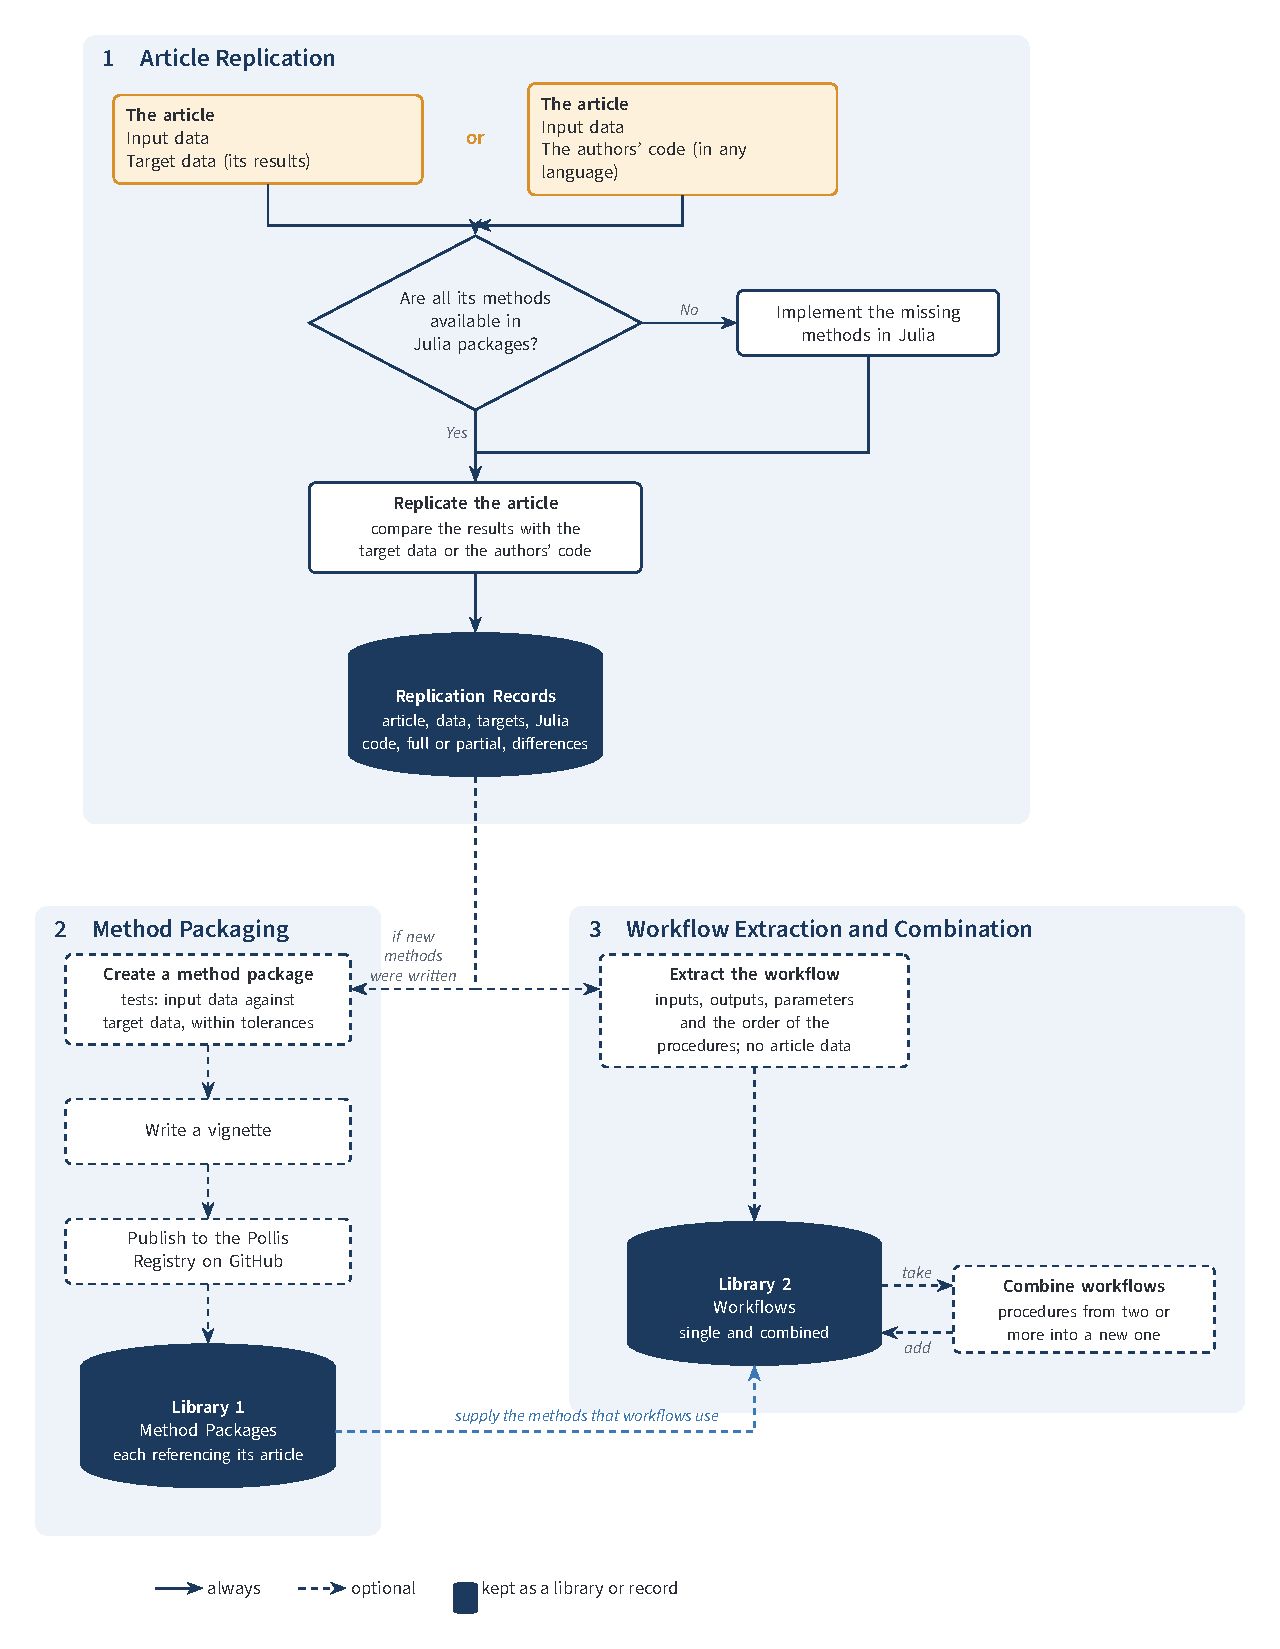
\includegraphics[width=\linewidth]{../workflows/replication_flowchart.pdf}
\end{minipage}\hfill
\begin{minipage}[t]{0.365\linewidth}\vspace{0pt}
\begin{pbox}{Replication}
It starts from an article, its input data, and either its published results or its authors' code,
in any language. If a method is missing from Julia's packages, it is written first. Each result is
printed beside the published one. A replication
record keeps the article, its data, the targets, the Julia code, whether the replication is full or
partial, and any differences. Find the replications in \textbf{Compose \textrightarrow{} Replication}.
\end{pbox}
\vspace{1mm}
\begin{pbox}{Methods}
Here a method is something particular: one an article needed that no Julia package had. It becomes a
documented package whose tests run the article's data and check its results within tolerances, with
a vignette, published to the Pollis Registry.
\end{pbox}
\vspace{1mm}
\begin{pbox}{Workflows}
A workflow is extracted from a replication: it keeps the inputs, outputs, parameters and the order of
the procedures, without the article's data, so it runs again on your own data. Procedures from two or
more workflows can be combined into a new one, where independent procedures run side by side, in \textbf{Compose \textrightarrow{} Workflows}.
\end{pbox}
\end{minipage}

\vspace{1mm}
{\footnotesize\color{soft}\textbf{Next steps:} a General Composition Algebra, including nesting (workflows inside
workflows), automatic matching (which outputs fit which inputs, by meaning or by converting between types)
and versioning of sub-workflows.\par}
\vspace{0.5mm}
\begin{tcbraster}[raster columns=2, raster equal height, raster column skip=3mm, raster row skip=2mm]
\usecase[top=4pt, bottom=4pt]{chart-area}{Panel data}{Baltagi (2005)'s panel regressions, on Grunfeld's investment data,
  OECD gasoline demand and Munnell's public capital in the US states: pooled, fixed and random effects,
  table by table.\par\textrightarrow{} New Julia Package: \pkg{ErrorComponents.jl}}
\usecase[top=4pt, bottom=4pt]{chart-line}{Volatility}{Bollerslev and Ghysels (1996): a GARCH model with a calendar effect
  in the variance, on daily Deutschmark--pound returns from 1984 to 1991.\par\textrightarrow{} New Julia Package: \pkg{PeriodicGARCH.jl}}
\usecase[top=4pt, bottom=4pt]{heartbeat}{Survival}{Dickson, Grambsch, Fleming, Fisher and Langworthy (1989): the Mayo Clinic
  model for primary biliary cirrhosis, a Cox model with seven years of predicted survival.\par\textrightarrow{} New Julia Package: \pkg{BreslowCox.jl}}
\usecase[top=4pt, bottom=4pt]{rocket}{Risk}{Dalal, Fowlkes and Hoadley (1989): the space shuttle's O-rings
  before the Challenger accident, a logistic regression of O-ring damage on launch temperature over 23 flights.\par\textrightarrow{} New Julia Package: \pkg{GLMExtras.jl}}
\end{tcbraster}

\vspace{1mm}
\begin{nbox}{New methods, with their proof attached}
Nine times, a paper needed a method that no Julia package had. Each is now a documented Julia
package, tested against the paper's tables or its authors' code, with a vignette, in
\textbf{Compose \textrightarrow{} Methods}, ready to use on your own data.
\end{nbox}

\newpage
% =====================================================================
% PAGE 9 — REPORTS
% =====================================================================
\pageheading{Reports}{From notebook to PDF.}
  {LaTeX reports and beamer slides from any notebook, with or without an agent.}

\begin{pbox}{Reports: from notebook to PDF}
Turn any notebook into a LaTeX report or a set of beamer slides with one click, from the Export button
on the notebook's toolbar or from \textbf{Compose \textrightarrow{} Reports}. Pollis runs the notebook and
writes its text, results and figures into a document, then compiles the PDF. No agent is needed. A
workflow can bring its own report template, laid out like the paper it replicates. When the data change,
export again: the numbers are refreshed and your edits are kept. If you like, your coding agent can then
polish the draft into a finished document, with sections, tables, captions and citations, using the
numbers already computed.
\end{pbox}

\vspace{4mm}
\begin{tcbraster}[raster columns=3, raster equal height, raster column skip=3mm]
\collabmode{Report}{}{Export Notebook as LaTeX.}{%
  \begin{itemize}[leftmargin=1em]
  \item The notebook's text, in a LaTeX article.
  \item What each cell prints, and each figure, in its place; the code stays in the notebook.
  \item Compiled to PDF, shown beside the source.
  \end{itemize}}
\collabmode{Slides}{}{Make Slides from a Notebook.}{%
  \begin{itemize}[leftmargin=1em]
  \item Beamer slides from the same notebook.
  \item A frame for the text under each heading, and one for each result and each figure.
  \item Ready to present, or to polish.
  \end{itemize}}
\collabmode{Polish}{optional}{Polish with Agent.}{%
  \begin{itemize}[leftmargin=1em]
  \item Your coding agent rewrites the draft: a title, an abstract, sections, tables and captions.
  \item It never retypes a number: every value comes from what Pollis computed.
  \item The PDF reloads beside you as it works.
  \end{itemize}}
\end{tcbraster}

\vspace{5mm}
\subhead{How a report is made}
\begin{enumerate}[label={\color{deepamber}\bfseries\arabic*}, leftmargin=5mm, itemsep=3pt]
  \small
  \item \textbf{The notebook runs.} Its code cells run in order, and what each prints and draws is saved
    beside the document; a workflow's template writes the tables and figures of its paper instead.
  \item \textbf{The draft is written once.} The \texttt{.tex} file is written only when there is none, so it is
    yours to edit from then on.
  \item \textbf{Export again, at any time.} New data or a changed step: the results and figures are refreshed,
    and your text stays as you left it.
  \item \textbf{The PDF is compiled in Pollis,} with Tectonic, through the \pkg{PollisTeX.jl} package: no separate LaTeX installation is needed.
\end{enumerate}

\vspace{5mm}
\begin{minipage}[t]{0.485\linewidth}\vspace{0pt}
\begin{pbox}[equal height group=p8pair]{Published values, side by side}
When a notebook replicates a paper, the polished report shows each published value beside the one Julia
computed, rounded to the published digits, with the page or table it comes from and how many decimals
they share. Where they differ, the report says so.
\end{pbox}
\end{minipage}\hfill
\begin{minipage}[t]{0.485\linewidth}\vspace{0pt}
\begin{pbox}[equal height group=p8pair]{Every reference, ready to cite}
Pollis keeps one library of every work its panels and notebooks refer to, 679 in all, as a single
BibTeX file. Reports cite from it as Author (year), with every author written out and a DOI link,
with nothing to copy.
\end{pbox}
\end{minipage}

\vspace{5mm}
\begin{nbox}{In one line}
Run the notebook, get the PDF, keep your edits: a report or slides in one click, polished by your agent if you like.
\end{nbox}

\newpage
% =====================================================================
% PAGE 10 — MONITOR: RSS FEEDS
% =====================================================================
\pageheading{Monitor}{Stay up to date, without searching.}
  {News, journals, central banks, podcasts and searches, read for you every hour.}

\begin{pbox}{RSS Feeds}
\textbf{Explore \textrightarrow{} Monitor \textrightarrow{} RSS Feeds} gathers what you follow in one page: financial news and markets,
central banks, the leading journals of statistics, economics, finance and medicine, new papers on arXiv,
medRxiv and bioRxiv, blogs on AI and Julia, podcasts and YouTube channels. Pollis reads every feed each hour, by
topic, and the newest unread items of the feeds you choose also appear on the welcome page, under \textbf{RSS}, where a camera or a microphone marks a video or a podcast. An item opens in
your browser; a video or an episode plays from its own \textbf{Watch} or \textbf{Listen} link. Nothing is read
for you by a server: the feeds come straight to your computer.
\end{pbox}

\vspace{4mm}
\begin{tcbraster}[raster columns=3, raster equal height, raster column skip=3mm]
\collabmode{Follow}{}{From a catalogue, or your own.}{%
  \begin{itemize}[leftmargin=1em]
  \item A catalogue of about 370 feeds sources in 35 categories, spanning History and Law, Music and Theatre, Physics and Medicine, with a sensible set followed from the start.
  \item An arXiv or PubMed search becomes a feed of the newest papers it finds.
  \item A YouTube channel, from its address or its @handle.
  \item A journal's page at Wiley, Taylor \& Francis, SAGE, Elsevier or Oxford Academic: Pollis finds its table-of-contents feed.
  \end{itemize}}
\collabmode{Read}{}{Only what you want to see.}{%
  \begin{itemize}[leftmargin=1em]
  \item Pictures and a short summary for each item.
  \item Tick, by feed or by topic: Subscribed, shown Here, on the Welcome Page.
  \item Show the last week, month or quarter, or everything kept.
  \item An item opened is marked read; \textbf{Mark Unread} marks it again.
  \end{itemize}}
\collabmode{Keep}{}{Your reading becomes data.}{%
  \begin{itemize}[leftmargin=1em]
  \item \textbf{Add to Zotero}: an article, preprint, video or episode goes to your library or collection, with its details, while Zotero is open.
  \item \textbf{Export as OPML}: follow the same feeds in Zotero or any feed reader.
  \item Every item is archived in the \textbf{PollisRSS} database, to query in Julia like any other.
  \end{itemize}}
\end{tcbraster}

\vspace{5mm}
\subhead{The PollisRSS database}
\begin{enumerate}[label={\color{deepamber}\bfseries\arabic*}, leftmargin=5mm, itemsep=3pt]
  \small
  \item \textbf{Every item, kept.} Each item read is added to a monthly archive on your computer, so nothing is lost when a feed drops it.
  \item \textbf{A built-in connection.} PollisRSS sits next to PollisDatasets in the Databases view; connecting it in the Julia REPL gives a DuckDB connection named \texttt{rss}.
  \item \textbf{Four views.} \texttt{items} holds every item, with its feed, topic, title, link, dates and summary; \texttt{feeds} sums them up by feed; \texttt{zotero} lists the items added to Zotero, and \texttt{episodes} the podcast episodes downloaded.
  \item \textbf{Then analyse it.} Count the papers on a topic month by month, find the authors who keep appearing, or measure how central-bank news moves with the markets.
\end{enumerate}

\vspace{5mm}
\begin{pbox}{Email Alerts}
Some services send the results of a saved search only by email: Google Scholar, JSTOR, HeinOnline, Nexis Uni, SSRN, Web of Science, Scopus, Westlaw, Factiva. Send them to an address of your own, and Pollis reads that mailbox on your computer and turns each alert into a feed, under \textbf{Add Feed \textrightarrow{} Email Alerts}, read and kept like any other; an agent skill writes precise searches for each source. Google Alerts and the publishers' table-of-contents alerts are feeds already, and Pollis follows them directly.
\end{pbox}

\vspace{5mm}
\begin{pbox}{Alerts on Quotes and SEC Filings}
\textbf{Explore \textrightarrow{} Alerts} warns you when a quote crosses a level, or when a company files a new 10-K, 10-Q or 8-K at the SEC's \textbf{EDGAR}, and keeps the second the filing was accepted. \textbf{Coming next, event studies:} at that second, Pollis fetches the company's 1-minute prices around the filing from Yahoo Finance, and keeps adding new ones as they come.
\end{pbox}

\vspace{5mm}
\begin{nbox}{In one line}
The news and research you follow, read every hour, kept as data, and one click from your Zotero library.
\end{nbox}

\newpage
% =====================================================================
% PAGE 11 — COLLABORATION
% =====================================================================
\pageheading{Collaboration}{Work together, from anywhere.}
  {Side by side or on the same page, with an agent if you like, and one day from your phone.}

\begin{pbox}{Collaboration}
Work together from wherever you are: two colleagues on different continents, or a tutor helping a student. Start a session, send the link and chat, with images; everything sent is enciphered. Then work in one of two ways, depending on how you like to work together. An agent can be invited to join the session too, and look at the code you share.
\end{pbox}

\vspace{2mm}
\begin{tcbraster}[raster columns=2, raster equal height, raster column skip=3mm]
\collabmode{Side by Side}{}{Pass the code. Share and compare.}{%
  \begin{itemize}[leftmargin=1em]
  \item Each of you keeps your own editor or notebook: any code file, or a Jupyter or Pluto notebook.
  \item You share it when you are ready. The others see your code next to their own, compare the two line by line, and copy yours with one click.
  \item Nobody can change anyone else's code.
  \item You share one editor at a time, when you choose.
  \end{itemize}}
\collabmode{Same Page}{next release}{Edit together. Live editing.}{%
  \begin{itemize}[leftmargin=1em]
  \item Everyone works on the same notebook or code at the same time.
  \item You see the others' changes as they type.
  \item The host opens a whole project folder to the others, who can browse and edit its files.
  \item Natural between close colleagues, and a bigger step of trust than Side by Side.
  \end{itemize}}
\end{tcbraster}

\vspace{4mm}
\begin{pbox}{Who works together}
\begin{itemize}[leftmargin=1.7em]
  \item[\listicon{\faUserFriends}] \textbf{Two people:} two colleagues, or a student and a tutor.
  \item[\listicon{\faUsers}] \textbf{A small group:} a research team, everyone sharing with everyone.
  \item[\listicon{\faChalkboardTeacher}] \textbf{A classroom:} students share with the tutor, and the tutor shares with the whole class.
  \item[\listicon{\faLayerGroup}] \textbf{Breakout groups:} a class split into teams, with the tutor visiting each one.
  \item[\listicon{\faChessKnight}] \textbf{A game:} teams and roles, private negotiations, and a facilitator who runs the simulation.
\end{itemize}
\smallskip
An agent can be invited to join any of them. The first version is for two people and small groups of up to five.
\end{pbox}

\vspace{4mm}
\begin{pbox}{Voice Link: collaborate on the move}
Coming later: your phone joins a session too. Driving to work, you think of a better way to run an analysis, and you just say it. Your phone sends your words, enciphered, to your own computer, where your agent takes the idea further with Pollis: it runs the panels, workflows and Julia code it needs, and saves a dated note of what it found in your Pollis Workspace. Your phone reads a short summary aloud: hands-free, with your eyes on the road. A colleague at another computer can join and add ideas too: you on the road, your agent and your colleague, on one idea from three places. When you arrive, it is all waiting on your computer.

\smallskip
\textbf{Above all, your agent knows your work.} Panels, Workflows and Views you selected and edited. The analyses, notes and reports you created. So the answer you hear is about your work, not a general one, and better than anything a chat without Pollis could give.
\end{pbox}

\newpage
% =====================================================================
% PAGE 12 — FREE, OPEN AND YOURS + GET STARTED  (message 4)
% =====================================================================
\pageheading{Free and open}{Free, open and yours.}
  {No licence fees, no lock-in, and code you can take anywhere.}

\begin{minipage}[t]{0.485\linewidth}\vspace{0pt}
\begin{itemize}[itemsep=3pt]
  \item[\color{deepamber}\faLockOpen] \textbf{Free and open source.} Pollis is licensed under the AGPL 3.0. The Julia packages it uses are open source too, most of them (259 of 289) under the permissive MIT licence; the others use BSD, Apache, Mozilla, GPL or AGPL licences.
  \item[\color{deepamber}\faDesktop] \textbf{Runs everywhere.} Windows, macOS and Linux.
  \item[\color{deepamber}\faCode] \textbf{A familiar editor.} Pollis is built on Code - OSS, the open-source core of VS Code, so it looks and works like a code editor many people already know.
  \item[\color{deepamber}\faPuzzlePiece] \textbf{Extensible.} It runs VS Code extensions and themes, from the Open VSX Registry or your own, and extensions can add new menus and panels (page 6). Extensions may use any licence.
\end{itemize}
\end{minipage}\hfill
\begin{minipage}[t]{0.485\linewidth}\vspace{0pt}
\begin{pbox}{What about AI?}
\begin{minipage}[t]{0.5\linewidth}\vspace{0pt}
AI is \textbf{off by default}, and Pollis works fully without it.
See \textbf{Pollis AI+} for Pollis and AI working together.
\end{minipage}\hfill
\begin{minipage}[t]{0.46\linewidth}\vspace{0pt}
\shot{images/shot_extensions.png}
\end{minipage}
\end{pbox}
\vspace{1mm}
% TODO (Antonio): confirm whether voice will be off by default like other AI features,
% and whether speech is processed on the computer or in the cloud, before adding either.
\begin{pbox}{Coming soon: voice \hspace{1.5mm}{\color{deepamber}\faMicrophone\hspace{1.5mm}\faVolumeUp}}
\textbf{Speak} commands, \textbf{dictate}, and \textbf{listen} to any panel read aloud,
with short texts written to be heard. Built on the latest VS Code voice features.
\end{pbox}
\end{minipage}

\vspace{4mm}
\begin{pbox}{Why Julia?}
Julia is free and open source, and it was designed for exactly this kind of work:
statistics, simulation and optimisation. Its code reads like the mathematics on the page
and runs fast without being rewritten in another language, so the code a panel gives you
is the code an expert would write. Its packages work together: a model from one can be
estimated, simulated or optimised with another. Python is larger and better known, and
Julia can call Python and R libraries when they are needed.\textsuperscript{1}\par\smallskip
{\footnotesize\color{soft}\textsuperscript{1}\,The first time you use a package, Julia prepares it for use.
This may take a few seconds for small packages and longer for larger ones; subsequent starts are much faster.}
\end{pbox}

\vspace{5mm}
\begin{nbox}{Get started in three steps}
\begin{minipage}[t]{0.70\linewidth}
\begin{enumerate}[label={\color{amber}\bfseries\arabic*}, leftmargin=5mm, itemsep=2pt]
  \item \textbf{Download} Pollis for your system: \textcolor{amber}{\downloadlink}
  \item \textbf{Install Julia} from the Welcome page: click \emph{Install Julia}.
  \item \textbf{Open a panel} from any menu, click \emph{Install} if it asks for packages,
    then press \emph{Julia REPL} and watch the example run.
\end{enumerate}
\end{minipage}\hfill
\begin{minipage}[t]{0.25\linewidth}\vspace{0pt}\centering
\colorbox{white}{\color{black}\qrcode[height=18mm]{https://github.com/saragga/pollis/releases/latest}}\par\vspace{2pt}
{\footnotesize Download Pollis}
\end{minipage}
\end{nbox}

\vspace{5mm}
\begin{minipage}[t]{0.485\linewidth}\vspace{0pt}
\begin{pbox}[equal height group=p7pair]{Work in progress}
Pollis is new. It works today, and its panels are being reviewed one by one,
with the key points of each panel being rewritten.
Found a problem, or missing a method? Use \textbf{Help \textrightarrow{} Report Issue} or
\textbf{Search Feature Requests}.
\end{pbox}
\end{minipage}\hfill
\begin{minipage}[t]{0.485\linewidth}\vspace{0pt}
\begin{pbox}[equal height group=p7pair]{The name}
\textbf{Pollis} echoes the Greek \emph{polis}, the community of citizens and the rules it
freely adopts. Like a polis, Pollis is shared: free, open source, built on open-source
packages, and open to change by those who use it. Its double \emph{l} recalls the Greek
\emph{poll\'a}, ``many things'': many fields and many methods in one place,
intertwined in a code that turns knowledge into action.
\par\medskip{\centering
\includegraphics[width=36mm]{images/wordmark.pdf}\par}
\end{pbox}
\end{minipage}

\vfill
\begin{minipage}[b]{0.70\linewidth}\small\color{soft}
\textbf{Thanks.} Pollis stands on the work of the Julia language, Code - OSS and the authors
of 289 open-source Julia packages.
\end{minipage}\hfill
\begin{minipage}[b]{0.26\linewidth}\raggedleft\small
\pollislogo{9mm}\par\vspace{2pt}
\textbf{Antonio Saragga Seabra}\\
\faEnvelope\ \contactemail
\end{minipage}

\newpage
% =====================================================================
% PAGE 13 — EVERYTHING IN POLLIS, AT A GLANCE (back cover)
% =====================================================================
\thispagestyle{empty}
\begin{tikzpicture}[remember picture, overlay]
  \fill[navy] (current page.south west) rectangle (current page.north east);
\end{tikzpicture}%
\newcommand{\mhead}[2]{{\color{amber}\fontsize{15}{17}\selectfont\bfseries #1}\hfill
  {\color{amber!75}\fontsize{9}{11}\selectfont #2}\par\vspace{3pt}
  {\color{amber!60}\rule{\linewidth}{0.6pt}}\par\vspace{5pt}}
\newcommand{\tbhead}[1]{{\color{amber}\fontsize{9.5}{11}\selectfont\bfseries #1}\par\nointerlineskip\vspace{3pt}
  \noindent{\color{amber!60}\rule{\linewidth}{0.5pt}}\par\vspace{2pt}}
\newenvironment{mcol}[1]{\begin{minipage}[t]{#1}\vspace{0pt}\raggedright\color{white}%
  \fontsize{8.6}{10.3}\selectfont\setlength{\parskip}{1.5pt}\everypar{\hangindent=2.5mm}}{\end{minipage}}
\newcommand{\entries}[1]{#1 entries}
% an item with a submenu, and an item shown with its submenu open
\newcommand{\sub}{\,{\color{amber}\fontsize{10.5}{10}\selectfont\bfseries ›}}
% the menu item shown open: amber, with a down chevron, remembered for the connector
\newcommand{\openitem}[1]{\tikz[remember picture, baseline=(rl.base)]\node[inner sep=0pt, text=amber,
  font=\bfseries](rl){#1\,\faAngleDown};}
% the magnifier box with the open submenu
\newcommand{\lensbox}[2]{%
  \tikz[remember picture]\node[inner sep=7pt, draw=amber, line width=0.9pt, rounded corners=6pt,
    fill=navy!80!black, text width=51mm, align=left](lens){%
    \raggedright{\color{amber}\bfseries\faSearchPlus\enspace #1}\par\vspace{4pt}
    {\raggedright\color{cream}\fontsize{8.4}{10.2}\selectfont\setlength{\parskip}{1.5pt}#2}};}

% The logo, framed in amber so it shows on the navy page, as tall as the title and the counts line
\newsavebox{\everyhead}
\sbox{\everyhead}{\begin{minipage}[c]{0.84\linewidth}
  {\color{white}\fontsize{30}{34}\selectfont\bfseries Everything in Pollis}\par\vspace{4pt}
  {\color{amber}\normalsize 5 curated menus\enspace·\enspace 203 method panels\enspace·\enspace 656 procedures\enspace·\enspace 289 open-source Julia packages}
\end{minipage}}
\newlength{\everyheadh}\setlength{\everyheadh}{\dimexpr\ht\everyhead+\dp\everyhead\relax}
\noindent\begin{tikzpicture}[x=\everyheadh/512,y=-\everyheadh/512,baseline=(current bounding box.center)]
    \draw[amber,line width=0.8pt,rounded corners=2mm] (0,0) rectangle (512,512);
    \fill[logodark] (36,422) -- (104,256) -- (172,422) -- cycle;
    \fill[logoamber] (104,422) -- (203,180) -- (302,422) -- cycle;
    \fill[logocream] (203,422) -- (339,89) -- (476,422) -- cycle;
  \end{tikzpicture}\hspace{3mm}\usebox{\everyhead}\par\vspace{3pt}
\hspace*{\dimexpr\everyheadh+3mm\relax}{\color{cream}\small Items marked {\color{amber}\bfseries\large ›} open a submenu; one is shown open.}

\vspace{5mm}
\begin{mcol}{0.29\linewidth}
\mhead{Explore}{\entries{50}}
Access Data Libraries\sub\par
Access Files and Databases\sub\par
Monitor\sub\par
Visualise\sub\par
Descriptive Statistics\par
Detect Anomalies\sub\par
Detect Novelties\par
Handle Missing Data\par
Interpolate Data
\end{mcol}\hfill
\begin{mcol}{0.36\linewidth}
\mhead{Model}{\entries{69}}
Model Evaluation\sub\par
Distributions\sub\par
Copulas\sub\par
Hypothesis Testing\par
Linear Models\sub\par
Linear Mixed Models\par
Generalised Linear Models\par
Generalised Linear Mixed Models\par
Nonlinear Regression\par
Penalised and Projection Regression\par
Robust and Quantile Regression\par
Time-Series Forecasting\par
State-Space Inference Methods\par
System Identification Methods\par
ODE Inference Methods\par
Nonlinear Dynamics\sub\par
Point Processes\par
Survival Analysis\sub\par
Bayesian Analysis\sub\par
Decision Trees\par
K-Nearest Neighbours\par
Rule-Based Methods\par
Neural Network Architectures\sub\par
Ensemble Learning Methods\par
Clustering\sub\par
Dimensionality Reduction Methods\sub\par
Natural Language Processing\sub
\end{mcol}\hfill
\begin{mcol}{0.29\linewidth}
\mhead{Simulate}{\entries{26}}
Sampling Foundations\sub\par
Markov Chain Monte Carlo\par
Sequential Monte Carlo\par
Multilevel Monte Carlo\par
Bootstrap Resampling\par
Probabilistic Programming Languages\sub\par
Uncertainty Propagation\par
Point Processes\par
State Space Models\par
Continuous Dynamical Systems\par
Discrete Maps\par
Stochastic Differential Equations\sub\par
Agent-Based Simulation\sub\par
Network Models\sub\par\vspace{6mm}
\hspace*{-7mm}\lensbox{Reinforcement Learning}{Bandit Problems\par
Q-Learning\par
Policy Gradient Methods\par
Actor-Critic Methods\par
Multi-Agent Reinforcement Learning\par
AlphaZero}
\end{mcol}

\vspace{3mm}
\begin{minipage}[t]{0.475\linewidth}\vspace{0pt}
\tikz[remember picture,overlay]\coordinate(opt);{\color{white}\mhead{Optimise}{\entries{51}}}
\begin{mcol}{0.485\linewidth}
Gradient-Free Optimisation\sub\par
Gradient-Based Optimisation\sub\par
Stochastic and Learning-Based Optimisation\sub\par
Global Optimisation\sub\par
Bayesian Optimisation\par
Surrogate-Based Optimisation\par
Evolutionary Computation\sub\par
Swarm Intelligence\par
Optimisation on Riemannian Manifolds\par
Discrete and Combinatorial Optimisation\par
Network and Graph Optimisation\par
Multi-Objective Optimisation\sub\par
Linear Programming\par
Quadratic Programming\par
Polynomial Programming\par
Convex, Conic and Semidefinite Programming\sub
\end{mcol}\hfill
\begin{mcol}{0.485\linewidth}
Nonlinear Programming\par
Hierarchical Optimisation\par
Complementarity and Variational Problems\sub\par
Uncertainty-Set Robust Optimisation\par
Chance-Constrained and Distributionally Robust\par
Stochastic Programming\par
Dynamic Programming\par
Optimal Control\sub\par
Markov Decision Processes\sub\par
\openitem{Reinforcement Learning}\par
Infinite-Dimensional Optimisation
\end{mcol}
\end{minipage}\hfill
\begin{minipage}[t]{0.475\linewidth}\vspace{0pt}
\tikz[remember picture,overlay]\coordinate(tb);\mhead{Compose}{13 entries}
\begin{mcol}{0.485\linewidth}
Local Models\sub\par
Coding Agents\par
Agent Skills\par
Orchestration\sub\par
New Panels and Toolboxes\sub\par
Replication\sub\par
Methods\sub
\end{mcol}\hfill
\begin{mcol}{0.485\linewidth}
Workflows\sub\par
Reports\sub\par
Correctness Tests\sub\par
Profiling\sub\par
Compilation Lab\sub\par
Collaboration\sub
\end{mcol}\par\vspace{8pt}
{\color{cream}\fontsize{8.4}{10.2}\selectfont Compose goes beyond single panels: a coding agent and its skills, local reasoning models, new methods,
analytical and operational workflows, reports, tests and collaboration. Toolboxes add their own menus
(page 7).}
\end{minipage}

\begin{tikzpicture}[remember picture, overlay]
  \path let \p1=(tb), \p2=(opt) in coordinate (g) at (\x1-4mm, \y2+6.3mm);
  \draw[amber, line width=0.9pt, rounded corners=3pt, -{Latex[length=2.2mm]}]
    (lens.south) |- (g) -- (g |- rl.east) -- ([xshift=1.2mm]rl.east);
\end{tikzpicture}%
\vfill
{\centering
{\color{cream}\Large Bright Insights through Statistical Learning, Simulation and Optimisation}\par\vspace{4pt}
{\color{amber!80}\small Pollis\enspace·\enspace free and open source\enspace·\enspace Windows, macOS, Linux\enspace·\enspace \faDownload\ \downloadlink\enspace·\enspace \faEnvelope\ \contactemail}\par\vspace{2pt}
{\color{amber!60}\footnotesize A Tour of Pollis, dated \tourdate}\par}

\end{document}
